% This template has been tested with LLNCS DOCUMENT CLASS -- version 2.20 (24-JUN-2015)

%"runningheads" enables:
%  - page number on page 2 onwards
%  - title/authors on even/odd pages
%This is good for other readers to enable proper archiving among other papers and pointing to
%content. Even if the title page states the title, when printed and stored in a folder, when
%blindly opening the folder, one could hit not the title page, but an arbitrary page. Therefore,
%it is good to have title printed on the pages, too.
\documentclass[runningheads,a4paper]{llncs}[2015/06/24]

\makeatletter
\renewcommand\paragraph{\@startsection{paragraph}{4}{\z@}%
            {-2.5ex\@plus -1ex \@minus -.25ex}%
            {1.25ex \@plus .25ex}%
            {\normalfont\normalsize\bfseries}}
\makeatother
\setcounter{secnumdepth}{2} % how many sectioning levels to assign numbers to
\setcounter{tocdepth}{4}    % how many sectioning levels to show in ToC

%cmap has to be loaded before any font package (such as cfr-lm)
\usepackage{cmap}
\usepackage[T1]{fontenc}

\usepackage{graphicx}
\graphicspath{ {images/} }

%Even though `american`, `english` and `USenglish` are synonyms for babel package (according to https://tex.stackexchange.com/questions/12775/babel-english-american-usenglish), the llncs document class is prepared to avoid the overriding of certain names (such as "Abstract." -> "Abstract" or "Fig." -> "Figure") when using `english`, but not when using the other 2.
%english has to go last to set it as default language
\usepackage[ngerman,english]{babel}
%Hint by http://tex.stackexchange.com/a/321066/9075 -> enable "= as dashes
\addto\extrasenglish{\languageshorthands{ngerman}\useshorthands{"}}

%better font, similar to the default springer font
%cfr-lm is preferred over lmodern. Reasoning at http://tex.stackexchange.com/a/247543/9075
\usepackage[%
rm={oldstyle=false,proportional=true},%
sf={oldstyle=false,proportional=true},%
tt={oldstyle=false,proportional=true,variable=true},%
qt=false%
]{cfr-lm}
%
%if more space is needed, exchange cfr-lm by mathptmx
%\usepackage{mathptmx}

%for demonstration purposes only
\usepackage[math]{blindtext}

%Sorts the citations in the brackets
%It also allows \cite{refa, refb}. Otherwise, the document does not compile.
%  Error message: "White space in argument"
\usepackage{cite}
\usepackage[mathletters]{ucs}
\usepackage[utf8x]{inputenc}

\usepackage{amsmath}
\usepackage{algorithm}
\usepackage[noend]{algpseudocode}

\makeatletter
\def\BState{\State\hskip-\ALG@thistlm}
\makeatother


%% If you need packages for other papers,
%% START COPYING HERE
%% COPY ALSO cmap and fontenc from lines 10 to 12

%extended enumerate, such as \begin{compactenum}
\usepackage{paralist}

%put figures inside a text
%\usepackage{picins}
%use
%\piccaptioninside
%\piccaption{...}
%\parpic[r]{\includegraphics ...}
%Text...

%for easy quotations: \enquote{text}
\usepackage{csquotes}

%enable margin kerning
\usepackage{microtype}

%tweak \url{...}
\usepackage{url}
%\urlstyle{same}
%improve wrapping of URLs - hint by http://tex.stackexchange.com/a/10419/9075
\makeatletter
\g@addto@macro{\UrlBreaks}{\UrlOrds}
\makeatother
%nicer // - solution by http://tex.stackexchange.com/a/98470/9075
%DO NOT ACTIVATE -> prevents line breaks
%\makeatletter
%\def\Url@twoslashes{\mathchar`\/\@ifnextchar/{\kern-.2em}{}}
%\g@addto@macro\UrlSpecials{\do\/{\Url@twoslashes}}
%\makeatother

%diagonal lines in a table - http://tex.stackexchange.com/questions/17745/diagonal-lines-in-table-cell
%slashbox is not available in texlive (due to licensing) and also gives bad results. This, we use diagbox
%\usepackage{diagbox}

%required for pdfcomment later
\usepackage{xcolor}


%enable nice comments
%this also loads hyperref
\usepackage{pdfcomment}
%enable hyperref without colors and without bookmarks
\hypersetup{hidelinks,
   colorlinks=true,
   allcolors=black,
   pdfstartview=Fit,
   breaklinks=true}
%enables correct jumping to figures when referencing
\usepackage[all]{hypcap}

\newcommand{\commentontext}[2]{\colorbox{yellow!60}{#1}\pdfcomment[color={0.234 0.867 0.211},hoffset=-6pt,voffset=10pt,opacity=0.5]{#2}}
\newcommand{\commentatside}[1]{\pdfcomment[color={0.045 0.278 0.643},icon=Note]{#1}}

%compatibality with packages todo, easy-todo, todonotes
\newcommand{\todo}[1]{\commentatside{#1}}
%compatiblity with package fixmetodonotes
\newcommand{\TODO}[1]{\commentatside{#1}}

%enable \cref{...} and \Cref{...} instead of \ref: Type of reference included in the link
\usepackage[capitalise,nameinlink]{cleveref}
%Nice formats for \cref
\crefname{section}{Sect.}{Sect.}
\Crefname{section}{Section}{Sections}

\usepackage{xspace}
%\newcommand{\eg}{e.\,g.\xspace}
%\newcommand{\ie}{i.\,e.\xspace}
\newcommand{\eg}{e.\,g.,\ }
\newcommand{\ie}{i.\,e.,\ }

%introduce \powerset - hint by http://matheplanet.com/matheplanet/nuke/html/viewtopic.php?topic=136492&post_id=997377
\DeclareFontFamily{U}{MnSymbolC}{}
\DeclareSymbolFont{MnSyC}{U}{MnSymbolC}{m}{n}
\DeclareFontShape{U}{MnSymbolC}{m}{n}{
    <-6>  MnSymbolC5
   <6-7>  MnSymbolC6
   <7-8>  MnSymbolC7
   <8-9>  MnSymbolC8
   <9-10> MnSymbolC9
  <10-12> MnSymbolC10
  <12->   MnSymbolC12%
}{}
\DeclareMathSymbol{\powerset}{\mathord}{MnSyC}{180}

% correct bad hyphenation here
\hyphenation{op-tical net-works semi-conduc-tor}

%% END COPYING HERE


\begin{document}

\title{Ensemble Method for Time Series Forecasting}
%If Title is too long, use \titlerunning
%\titlerunning{Short Title}

%Single insitute
\author{Aleksandar Bachvarov \and Atanas Dimitrov}
%If there are too many authors, use \authorrunning
%\authorrunning{First Author et al.}
\institute{Karlsruhe Institute of Technology}

%Multiple insitutes
%Currently disabled
%
\iffalse
%Multiple institutes are typeset as follows:
\author{Firstname Lastname\inst{1} \and Firstname Lastname\inst{2} }
%If there are too many authors, use \authorrunning
%\authorrunning{First Author et al.}

\institute{
Insitute 1\\
\email{...}\and
Insitute 2\\
\email{...}
}
\fi
			
\maketitle

\begin{abstract}
Abstract goes here
\end{abstract}

\begin{keywords}
time series, forecasting, ensemble methods, machine learning, arbitrating  
\end{keywords}


\section{Introduction}\label{sec:intro}

\section{Fundamentals of time series forecasting}

	\subsection{Definition}
		\subsubsection{Time series}
		 \hspace{1cm}\\\\A time series is sequence of data points, which are ordered and indexed by time. The data presented in the series could be any variable capable for observation over time. Some examples of time series include the price of a specific stock, the height level of a river and the national birth rate over time. Time series could be presented by multiple ways: as a list of values, as a graph, as a bar chart etc. On  \hyperref[fig:bitcoin]{Fig. \ref{fig:bitcoin}} you can see a graph of the bitcoin price time series over the last year. Beside investing, time series is used in many other fields like e.g. statistics, insurance, weather forecasting, astronomy, applied  science and many more.
		
\begin{figure}[h]
\centering
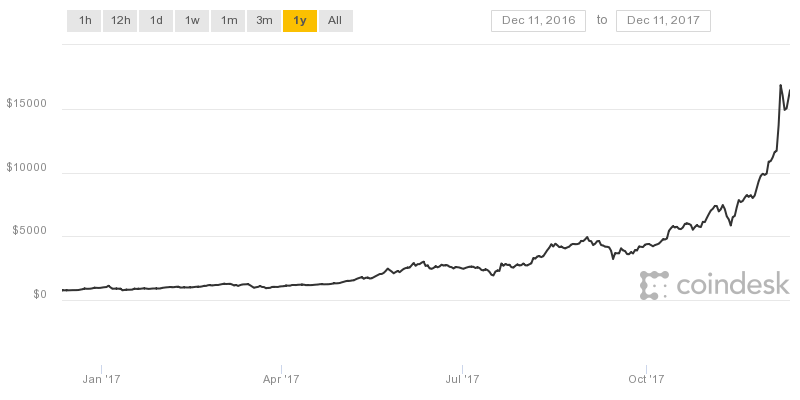
\includegraphics[width=\textwidth]{bitcoin}
\caption{Bitcoin price history from December,  2016 to December, 2017.}
\label{fig:bitcoin}
\end{figure}

		\subsubsection{Forecasting} \hspace{1cm}\\\\Time series forecasting represents the process of predicting the future values of the observed variable based on the already available data. In order to achieve that, dependencies among the available time series must be found, which then approximate the possible future values. Various methods were used over the years. They are in general divided  in two groups: linear and non-linear methods. The most significant of them will be wider presented  further in this paper. It's important to be noted that time series forecasting is just forecasting - the purpose is that the forecast is as close as possible to the future value, but there is no warranty for that. Generally applies that the deviation of the forecast increases with his time distance.\\\\ Time series could be not-stationary (volatile) or stationary. In other words - to have higher or lower degree of stationarity. The distribution of the stationary one depends much more on a long term trend while the distribution of the not-stationary one - on occasional events. Example for an extremely stationary time series is the coin flipping over time, example for an extremely volatile one - the bitcoin price. Because of his characteristics the volatile time series is much harder to predict. His wide spread and importance led to the development of more complex (non-linear) methods for doing that. Those methods include and are based on some machine learning techniques like e.g. bagging and boosting and also on key machine learning tools like artificial neural networks. Time series forecasting is one of the classic and at the same time very important areas of the machine learning.
	\subsection{Origins and related topics}
		\subsubsection{Machine Learning}\hspace{1cm}\\\\ 
In the recent years, as many useful applications of machine learning have been developed and have become part of our everyday life, his significance increased. We hear more and more often the term on the news or read about it on the Internet. In many cases machine learning is used as a synonym for artificial intelligence (AI), which is incorrect. AI is field of computer science, which is studying and  applying approaches for making computers being able to execute cognitive tasks\cite{AIvsML}. Machine learning is one of those approaches and it's by far the most successful (widely used, with the most applications) one of them\cite{quinlan1986induction}. His subject is the studying and the computer modelling of learning processes.\cite{Michalski1983}. \\\\ One common way to create a new machine learning process is to research the human learning mechanisms, to adapt them and then accordingly to simulate them  with algorithms. The artificial neural networks (commonly utilized machine learning tool) are example for that and they will be discussed thoroughly further in the paper. It is  restrictive to believe that the learning patterns that come from the nature are the only possible way for acquiring knowledge. Reserchers also try to manifacture their own ones. By doing this main criteria are the methods'  generality and performance rather than their psychological explanation\cite{Michalski1983}.\\\\ 
In order to better understand one single learning methodology, we classify it by some meaningful parameters:
\begin{enumerate}
\item the amount of inference performed on the available information
\item the representation of knowledge acquired by the learner. 
\item the application domain of the collected knowledge 
\end{enumerate}\hspace{1cm}\\Different amount of inference means that the learning system analyses the data more or less and makes more or less interdependencies between it. Example for no inference is the simple remembering of facts with no thoughts about them and any other already existing knowledge. Example for middle range inference is the learning from teacher or book that provides the learner positive and negative examples. The learner analyses the input data and makes some conclusion about it based mainly on his already existing knowledge. Example for extremely high level of inference is the learning from observation and the discovery. There is no source of certain information to learn from and the learner should discover it alone\cite{Michalski1983}. The high and the low level of inference of learning methods has both their pluses and minuses - it's much harder and slower to learn something just by yourself, but therefore you reach deeper understanding of the topic. When the learner is a real person and not a computer algorithm, it could be even dangerous for him. My driving instructor used to tell me that I can always learn to drive by myself, but to achieve it, I must break at least three cars. In order to prevent that he was there to teach me.\\\\
There are a lot of different representations of knowledge that the learner can produce. Some popular examples include the decision trees that will be discussed in detail, parameters in algebraic expressions, formal grammars, graphs, computer programs, classification categories etc.\\\\
We know from the near past and the present  (and for sure will hear more about it in the future) that the machine learning has a lot of applications. Some popular application domains of the learners are the self driving cars, speech and face recognition, the expert systems and of course - the subject of our paper - time series forecasting.  \\\\As next on this paper follow some presentation of key tools and techniques in machine learning at all and in the field of time series forecasting specifically.
				
\paragraph{Decision trees}
 A decision tree could be defined as form of classification or regression rule that a learner has inducted after his feeding with data. Let's assume we have a set of objects. All these objects have attributes, which  have values. Besides that we also know that each object belongs to one specific class and there are at least two different classes. From that data a decision tree could be inducted. Latter we can use that decision tree for classification - defining to which of the classes any object belongs. Under \enquote{any} here are all objects from the same type as the input objects to be understand. The regression decision tree is similar to the classification one - the difference is that the delight output isn't class label as by classification, but it's a continuous value. For better understanding we will stay on the classification in the further explanations\cite{quinlan1986induction}.\\\\It must be said that the decision tree is used for predictions. In that matter there is no 100\% warranty that the prediction true. In order to increase the probability for correct forecast, we must first select as less redundant data as possible. With other words that selected objects must cover the whole spectrum of different objects, but with no duplicates. When this condition isn't fulfilled, we have the so called underfitting\cite{quinlan1986induction}.\\\\
Even without underfitting there are still chance that the decision tree doesn't return the correct class label. This may be caused by overfitting - when the decision tree corresponds too much to the training data, but isn't abstract enough (doesn't return correct class labels for other data). In order to fix that problem many ensemble techniques could be used. One of them is the so called \enquote{Random forest}. A random forest is a set of different decision trees that we have generated through e.g. sampling. In order to determine the output value, we chose the mode of the selected classes from all trees in the forest\cite{breiman2001random}.\\\\
An example decision tree is given on \hyperref[fig:decisionTree]{Fig. \ref{fig:decisionTree}}. It represents the classification of whether or not you should give credit to someone. The nodes are shown as conditions for the values of the object's attributes. The edges are signed with the possible values of the attributes and route the path of the selection. The leafs are the different class label. On the example we see that you will probably get credit, if you are first over 40 years old and own a house, because it will be mortgaged or if you earn enough money to cover your debt.   
    
\begin{figure}[h]
\centering
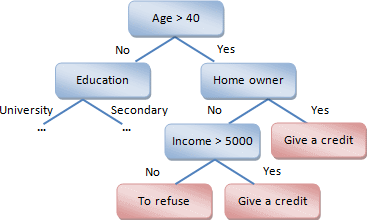
\includegraphics[width=\textwidth]{decisionTree}
\caption{Decision tree about whether to give credit to someone or not}
\label{fig:decisionTree}
\end{figure}
		 
\paragraph{Artificial Neural Networks}
	
The artificial neural networks are one of the widely employed tools in the machine learning. They simulate the learning and predicting activity of the brain. Similar to the process of teaching humans the artificial neural nets are trained with pairs of data - input variable and his corresponding result value according to the task. Then the net should be able to guess the output value of random input value that wasn't part of the training set. \\\\The  fundamental part of an artificial neural network is the model of the neuron. It consists of three elements\cite{haykin2009neural}:
\vspace{-\topsep}
\begin{enumerate}
\item set of synapses. Each synapse has a weight $w_{kj}$.  When passing through the synapse, the input signal $x_j$ is multiplied by his weight. The weight can hold positive and negative values.
\item an adder. Sums the multiplied input signals. 
\item an activation function. The sum of the adder's value and the bias $b_k$ goes as his argument. The function returns the output signal of the neuron. His purpose is to restrict the output signal between specific values e.g. -1 and 1.
\end{enumerate}
\vspace{-\topsep}

\begin{figure}[h]
\centering
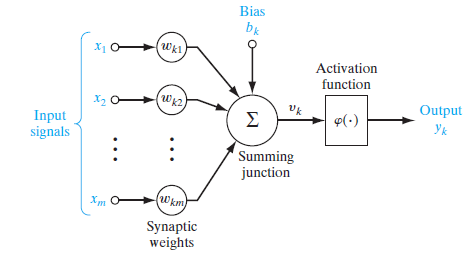
\includegraphics[width=\textwidth]{neuronModel}
\caption{Model of the artificial neuron $k$. Source: \cite{haykin2009neural}}
\label{fig:neuronModel}
\end{figure}

\hspace{1cm}\\ A scheme of the model could be seen on \hyperref[fig:neuronModel]{Fig. \ref{fig:neuronModel}}. Mathematically the neuron $k$ could be described with the following equations:

\begin{equation}
u_k = \sum_{j=1}^{m} w_{kj}x_j
\end{equation}

\begin{equation}
v_k = u_k + b_k
\end{equation}

\begin{equation}
y_k = φ(v_k)
\end{equation}Shortly explained the multiplication of all input signals $x_j$ with the weights $w_{kj}$ of their synapses are getting summed. This sum is then biased with $b_k$ and the result is put into the activation function $φ(.)$, which produce the output signal $y_k$.\\\\
The are some possibilities for activation function, but the mostly used are the sigmoid functions. A sigmoid function has a \enquote{S} shaped graph and and return value from 0 to 1 or from -1 to 1. One example is the logistic function.
\begin{equation}
φ(v) = \frac{1}{1 + exp(e^{-x})}
\end{equation}
One particular reason why the sigmoid functions are mostly employed as activation functions is the fact that they are differentiable. This quality is latter important for the backpropagation. \\\\The simplest neural net consist from only one neuron. Further, we can have many neurons in one single layer. In that  case the net is called single-layer feedforward network. If the net consists from more than one layer, then it's called multilayer feedforward network. Multilayer networks have an input layer, an output layer and could also a hidden layer or many of them. The ones with many hidden layers are called deep networks\cite{haykin2009neural}.

\begin{figure}[h]
\centering
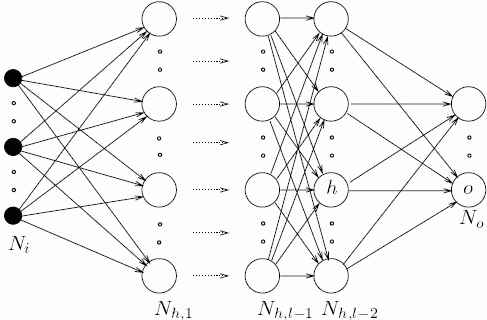
\includegraphics[width=\textwidth]{deepNetwork}
\caption{Schema of deep network: Source: \url{http://www.codeproject.com/KB/cs/BackPropagationNeuralNet/fig1_nnet_thinner.png}}
\label{fig:deepNetwork}
\end{figure}  
  
\hspace{1cm}\\ The ultimate goal of training each neural network is the adjusting of all weight values to such way that by passing an unknown input signal to the network, it will return a correct output signal. In order to achieve that a technique called backpropagation is used. Simply explained we need to pass an input signal through the network. Then we calculate the difference between the real expected value and the output value. With a special loss function and the difference as argument we calculate the new weight for each synapse and then adjust it by propagating the network backwards\cite{rumelhart1986learning}.\\\\ In order to employ the backpropagation the model have to fulfil two conditions. First, the activation function must be differentiable. The logistic function fulfils that. Second, there has to be no addition of $u_k$ with the bias, but at the same time the effect of the bias must be kept. That's achieved by using an extra dummy synapse with weight $w_{k0} = b_k$ and an input signal equals 1 or -1\cite{haykin2009neural}.
		 \paragraph{Ensemble Techniques}
		\subsubsection{General time series forecasting methods}
\section{Arbitrated Ensemble for Time Series Forecasting} In this section we will present a relatively new method for time series forecasting, which by far gives the most accurate results in comparison to older state-of-the-art methods. It was introduced by a team of Portuguese scientists on the European Conference on Machine Learning that took place on 18-22 September 2017 in Skopje, Macedonia. 

\subsection{General explanation}
Many forecasting methods use combination of different forecasters in order to achieve better accuracy by reducing the overfitting effect. So does the method of arbitrated ensemble as well. It assumes that every forecaster has his own expertise and has to be as diverse as possible. Due to the volatility and the seasonality of time series this unique expertise isn't equally distributed over time - some forecasters are more accurate at specific time (more precisely with input data with specific characteristics), other forecasters - at other specific time. Hence, we must build an ensemble of forecasters by first - weighting them according to their expertise on the specific situation - and second - summing the products of each forecaster and his expertise weight \cite{VtorCerqueira2017}. \\\\That leads us to the second essence of the presented method - the arbitrating or the arbitrating architecture. To arbitrate means in our case to decide how important is each forecaster for the final prediction. This happens through a second level of forecasters called meta-learners. Each main forecaster (or learner) has his own meta-learner. The meta-learner predicts the possible error of his learner according to the current input data characteristics. Those error values are latter  translated to forecaster's weights using  softmax function. The greater the predicted error is, the less the weight of the forecaster will be \cite{VtorCerqueira2017}.
\vspace{-\topsep}

\begin{figure}[h]
\centering
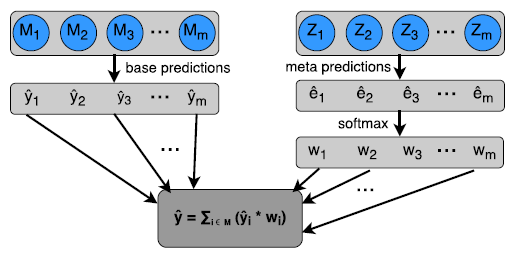
\includegraphics[width=\textwidth]{adeSchema}
\caption{Schema of the Arbitrated Dynamic Ensemble (ADE). $M_1, ... ,M_m$ are the main forecasters. They produce the predictions $y_1, ... ,y_m$. The meta-forecasters $Z_1, ... ,Z_m$ predict the error values $e_1, ... ,e_m$ of each main forecaster. From those errors the expertise weights $w_1, ... ,w_m$ are generated. At last the weights are used to calculate the weighted average of the predictions. \cite{VtorCerqueira2017}}
\label{fig:adeSchema}
\end{figure} 
 
\vspace{-\topsep}
\hspace{1cm}\\ The above described process is called Arbitrated Dynamic Ensemble (ADE) by his authors. It's illustrated on \hyperref[fig:adeSchema]{Fig. \ref{fig:adeSchema}}. 

\subsection{Data preparation and Learning Basic-Level Models}
\subsection{Learning Meta-Level Models}
The layer of meta-learners or meta-forecasters has to be trained to arbitrate the importance of each learner for the current prediction. As it was already mentioned, each learner has his own expertise. The task of the learner's corresponding meta-learner is to measure his expertise for a specific situation. In order to do that it has to predict the estimated error of the learner for that situation. The  described strategy is based on an arbitrating architecture, which was originally used with classifies and not with regression forecasters \cite{ortega2001arbitrating}. We train the meta-learner by using data samples corresponding to the following model:\begin{equation}
e^j = f(I)
\end{equation} $e^j$ is the absolute error caused by $M^j$, $I$ are the past values of the time series and $f$ is the regression function.\\\\ At the training phase our first task is to produce the out-of-bag predictions (OOB). We will than use them to train the meta-learners once before the start of the actual prediction session and once every time after predicting $y_t+1$. So, to produce the OOB we split the training set into $\beta$ equal blocks. We train the learners $M$ with the first block of data and then test them with the second. Then we merge the first and the second block, train the learners with this new larger block and test them with the third block. The operation continues up to the last block.\\\\Instead of using all base learners by predicting, it's a common sense to use only the best of them. We call the used learners the Committee of Models for Prediction. It contains the $\alpha$\% of the best forecasters( the one with the lowest error) in the last $\Omega$ observations. This reduction saves computational power from retraining of meta-learners that have learners with very low weight. Nevertheless, no matter whether his base learner is part of the committee of models or not, each meta-learner is trained on each $\lambda$ iterations. You can see the meta-learning algorithm in \hyperref[alg:metalearning]{Algorithm  \ref{alg:metalearning}}.
    
\begin{algorithm}[h]

\caption{Metalearnig $Z$}\label{alg:metalearning}
\begin{algorithmic}[1]

\Require Available observations at runtime $Y_{ts}$; Embedding Dimension $K$; Training
Signal $\lambda$; meta-committee ${}^{\alpha}Z$
\State $\text{Embed $Y_{ts}$ into $Y_{ts}^{K}$} \rightarrow I$
\ForAll{$Z^{j} \in {}^{\alpha}Z \text{ and not trained in the last training signal $\lambda$ }$}
\State $\text{train $Z^{j}$ to model: $e^{j} = f(I)$}$
\EndFor
\State $\text{Return ${}^{\alpha}Z$}$
\end{algorithmic}
\end{algorithm}

\subsection{Predicting the next time series}
 After the Committee of the most accurate $\alpha$\% base learners ${}^{\alpha}M$  is determined, we use the corresponding meta-learners ${}^{\alpha}Z$ to predict their possible error $e^j$. Then we put these errors into the softmax function and thus we generate the base learner's weighs\cite{VtorCerqueira2017}. This process is explained by the following equation:
 \begin{equation}
w^{j}_{t+1} = \frac{exp(-e^{j})}{\sum_{j \in {}^{\alpha}M} exp(-e^{j})}
\end{equation} It's interesting fact the the softmax function is used for neural nets modelling. What's more, it wasn't used by far for error translation.\\\\ The last step of the prediction is the calculation of the weighted average by summing the products of all predictions of the committee with their weights:
 \begin{equation}
y_{t+1} = \sum_{j \in {}^{\alpha}M} y^{j}_{t+1}.w^{j}_{t+1}
\end{equation}You can see the predicting $y_{t+1}$ algorithm in \hyperref[alg:predicting]{Algorithm  \ref{alg:predicting}}.


\begin{algorithm}[h]
\caption{Predicting $y_{t+1}$}
\label{alg:predicting}
\begin{algorithmic}[1]
\Require $K, M, Z,\alpha, \Omega, {}^{\alpha}M, {}^{\alpha}Z$
\State $\text{Embed the previous $K-1$ values  into $Y_{t+1}^{K}$}$
\State $\text{Get meta-predictions $e^{j}_{t+1}$ from $Z^{j} \in {}^{\alpha}Z$}$
\State $\text{Compute weigths $w^{j}_{t+1} =  exp(-e^{j}_{t+1})/\sum_{Z^{j} \in {}^{\alpha}Z} exp(-e^{j}_{t+1})$}$
\State $\text{Get predictions $y^{j}_{t+1} $ from models $M^{j} \in {}^{\alpha}M$}$
\State $\text{Compute final predictions $y_{t+1} = \sum_{j=1}^{m} y^{j}_{t+1}.w^{j}_{t+1}$}$
\State $\text{Add $y_{t+1}$ to $Y_{ts}$}$
\State $\text{Update Committees ${}^{\alpha}M$ and ${}^{\alpha}Z$ according to $\alpha$ and $\Omega$}$
\State $\text{Return $y_{t+1}$ and go back to the metalearning step (Algorithm \ref{alg:metalearning})}$
\end{algorithmic}
\end{algorithm}
\subsection{Performance comparison with general time series forecasting methods}

\section{Conclusion and Outlook}

\subsubsection{Acknowledgments}

%%%%%%%%%%%%%%%%%%%%%%%%%%%%%%%%%%%%%%%%%%%%%%%%%%%%%%%%%%%%%%%%%%%%%%%%%%%%%%%
\bibliographystyle{splncs03}
\bibliography{paper}

%%%%%%%%%%%%%%%%%%%%%%%%%%%%%%%%%%%%%%%%%%%%%%%%%%%%%%%%%%%%%%%%%%%%%%%%%%%%%%%

\end{document}
